\chapter{ВЫПОЛНЕНИЕ ЗАДАНИЯ}
Необходимо разработать программу для ПЛК для управления автоматизированной
установкой в соответствии с описанием ее работы.

\textbf{Цель} --- Сделать программу для управления автоматизированной установкой в соответствии с описанием ее работы.

При выполнении ставятся следующие задачи:
\begin{enumerate}
    \item Внимательно ознакомиться с заданием
    \item Изучить алгоритм работы установки
    \item Изучить электрическую схему подключения
    \item Изучить пневматическую схему подключения
    \item Определить сигналы для выполнения исполнительных элементов
    \item Создать программу для управления установкой
\end{enumerate}

Автоматическая установка состоит из трех пневматических цилиндров, шести
датчиков положения (герконы), одного двигателя постоянного тока и световой
колонны. Всеми перемещениями механизмов и индикацией световой колонны
управляет ПЛК (программируемый логический контроллер/программируемое
реле). Используется ПЛК ОВЕН ПР200-24 1.X.
Для реализации панели оператора используется встроенный scada система.

\section{Виртуальная панель оператора}
Виртуальная панель оператора в scada системе представлена на рисунке \ref{fig:scada_panel}.
\begin{figure}[hb]
    \centering
    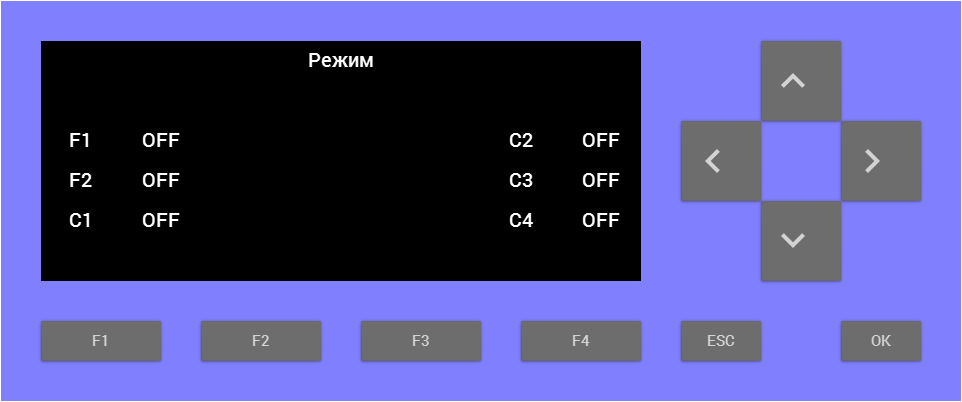
\includegraphics[width=1\textwidth]{fig/vpanel.png}
    \caption{Виртуальная панель оператора}
    \label{fig:scada_panel}
\end{figure}

\section{Описание клавиш панели оператора}
\begin{enumerate}
    \item F1 -- аварийный останов (1 – активация)
    \item F2 -- ручной/авто (0 – ручной, 1 – автоматический)
    \item F3 -- старт (авто) / движение выбранного цилиндра (ручной)
    \item F4 -- движение выбранного цилиндра (ручной)
    \item С1 -- выбор цилиндра 1 (ручной)
    \item С2 -- выбор цилиндра 2 (ручной)
    \item С3 -- выбор цилиндра 3 (ручной)
    \item С4 -- включение двигателя (ручной)
\end{enumerate}

Из кнопок F1, F2, С1, С2, С3, С4 необходимо сделать переключатели
программным способом.

\section{Условия запуска установки}
\begin{itemize}
    \item Штекер вставлен в розетку и ручной пневматический клапан открыт для подачи воздуха в систему.
    \item Все компоненты должны оставаться в своих стартовых позициях, цилиндры 1, 2 и 3 втянуты, двигатель выключен.
    \item Выбор режима работы автоматический/ручной может быть осуществлен переключателем F2.
    \item Установка начинает свою работу только если кнопка аварийного останова F1 не активирована.
\end{itemize}

\section{Аварийный останов}
В любой момент, при нажатии кнопки аварийного останова F1 прерывается
работа всех механизмов (цилиндры 1 и 2 втягиваются, цилиндр 3 остается в
текущем положении, двигатель выключается), механизмы не реагируют на
нажатия кнопок F2, F3, F4, С1, С2, С3, С4. Непрерывно горит красный
сигнал световой колонны. На виртуальном экране ПЛК отображается
актуальная информация о режиме и состояниях (ON/OFF) программных
переключателей F1, F2, С1, С2, С3, С4 на мигающем с частотой 1 Гц
красном фоне в формате, представленном на рисунке \ref{fig:alert_screen}.
Реализация режима представлена на рисунке \ref{fig:alert_mode}.
\begin{figure}[pt]
    \centering
    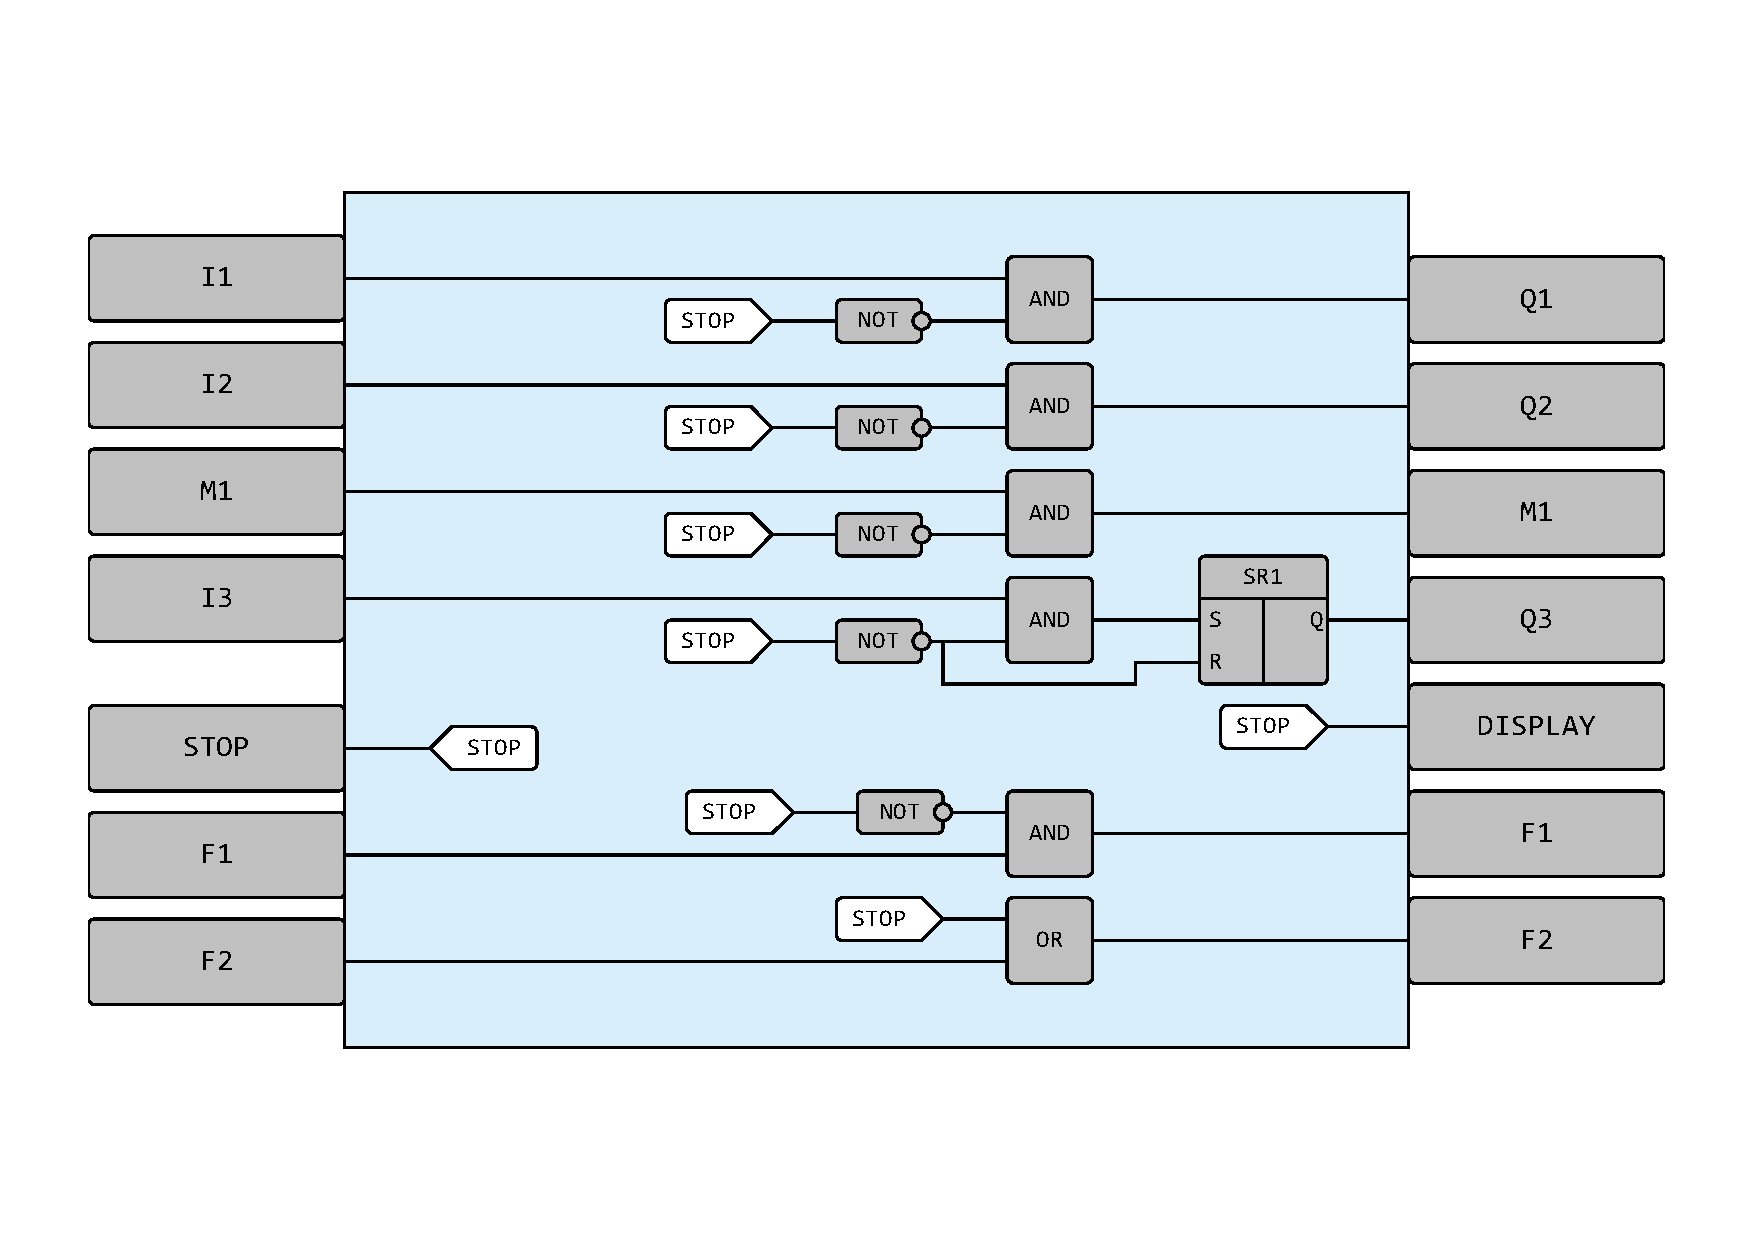
\includegraphics[width=1\textwidth]{fig/alert.pdf}
    \caption{Программа режима останова}
    \label{fig:alert_mode}
\end{figure}

\begin{figure}[pb]
    \centering
    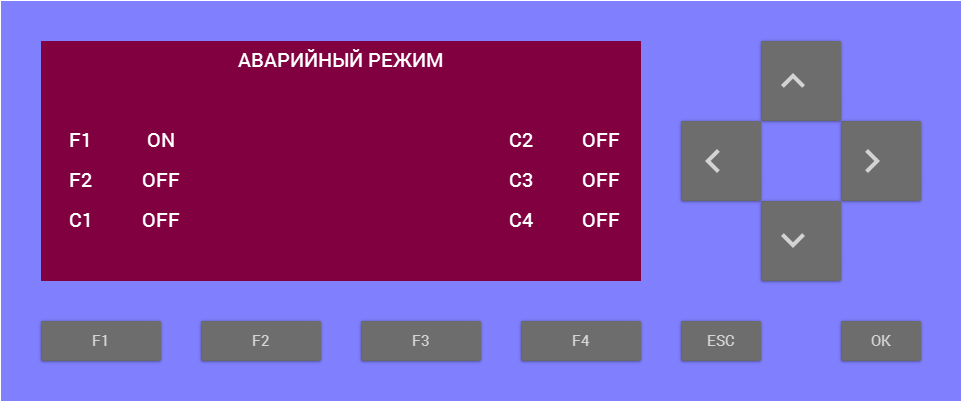
\includegraphics[width=1\textwidth]{fig/alert_panel.png}
    \caption{Экран режима аварийного останова}
    \label{fig:alert_screen}
\end{figure}


\newpage
\section{Автоматический режим}
Начальные условия: Цилиндры 1, 2 и 3 в стартовых позициях, двигатель
выключен. Переключатель F2 включен. Готовность системы к работе в
автоматическом режиме отображается миганием зеленого сигнала световой
колонны (~ 1 Гц).

Нажатие кнопки F3 запускает автоматический цикл:
\begin{enumerate}
    \item Зеленый сигнал световой колонны загорается непрерывно, включается двигатель и запускается таймер на 4 секунды
    \item Через 4 секунды цилиндр 3 выдвигается (засверливание первого отверстия)
    \item Когда цилиндр 3 выдвинут (3B2) цилиндр 1 выдвигается
    \item Когда цилиндр 1 выдвинут (1В2) цилиндр 3 втягивается
    \item Когда цилиндр 3 втянут (3B1) цилиндр 2 выдвигается
    \item Когда цилиндр 2 выдвинут (2В2) цилиндр 3 выдвигается (засверливание второго отверстия)
    \item Когда цилиндр 3 выдвинут (3B2) цилиндр 1 втягивается
    \item Когда цилиндр 1 втянут (1В1) цилиндр 3 втягивается
    \item Когда цилиндр 3 втянут (3B1) двигатель выключается, цилиндр 2 втягивается
    \item Когда цилиндр 2 втянут (2B1) зеленый сигнал световой колонны начинает мигать (~ 1 Гц). Автоматический цикл закончен.
\end{enumerate}

На виртуальном экране ПЛК отображается актуальная информация о
режиме и состояниях (ON/OFF) программных переключателей F1, F2, С1, С2,
С3, С4 на белом фоне в формате, представленном на рисунке \ref{fig:auto_screen}.
Реализация режима представлена на рисунке \ref{fig:auto_mode}.

\begin{figure}[pt]
    \centering
    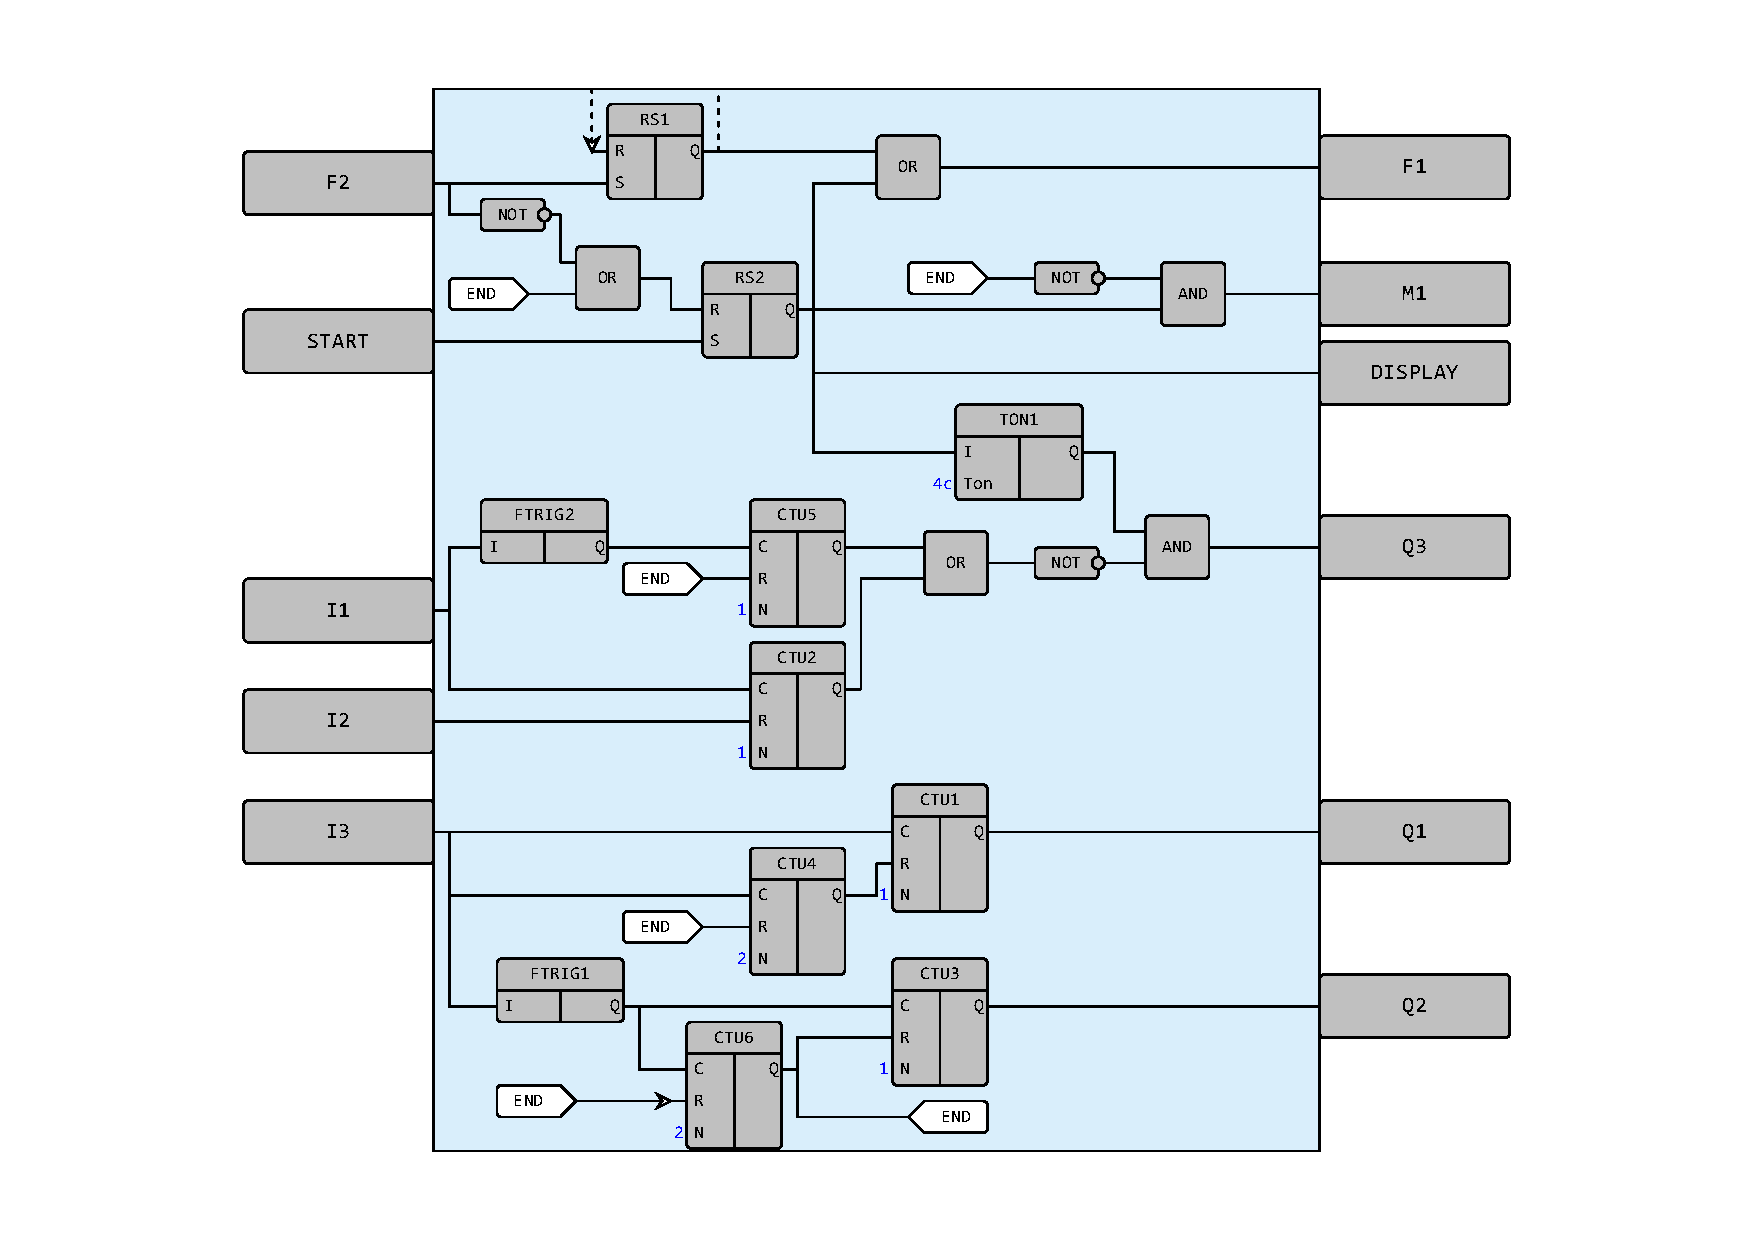
\includegraphics[width=1\textwidth]{fig/auto.pdf}
    \caption{Программа автоматического режима}
    \label{fig:auto_mode}
\end{figure}

\begin{figure}[pb]
    \centering
    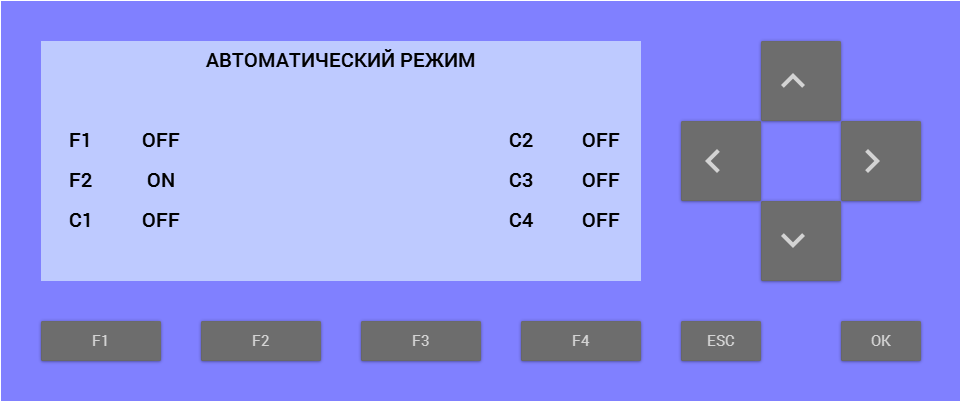
\includegraphics[scale=0.5]{fig/auto_panel.png}
    \caption{Экран автоматического режима}
    \label{fig:auto_screen}
\end{figure}


\newpage
\section{Ручной режим}
Начальные условия: Цилиндры 1, 2 и 3 в стартовых позициях, двигатель
выключен. Переключатель F2 выключен. Готовность системы к работе в ручном
режиме отображается непрерывно горящем желтым сигналом световой колонны.
В данном режиме перемещения механизмов независимы друг от друга и не
связаны циклической последовательностью действий.

\begin{itemize}
    \item Условие: переключатель C1 включен. При нажатии кнопки F3 цилиндр 1 выдвигается.
    \item Условие: переключатель C1 включен. При нажатии кнопки F4 цилиндр 1 втягивается.
    \item Условие: переключатель C2 включен. При нажатии кнопки F3 цилиндр 2 выдвигается.
    \item Условие: переключатель C2 включен. При нажатии кнопки F4 цилиндр 2 втягивается.
    \item Условие: переключатель C3 включен. При нажатии кнопки F3 цилиндр 3 выдвигается.
    \item Условие: переключатель C3 включен. При нажатии кнопки F4 цилиндр 3 втягивается.
    \item При включении переключателя C4 включается двигатель. К желтому сигналу светофора добавляется мигающий зеленый сигнал (1 Гц). Выключение переключателя C4 выключает двигатель.
\end{itemize}

На виртуальном экране ПЛК отображается актуальная информация о
режиме и состояниях (ON/OFF) программных переключателей F1, F2, С1, С2,
С3, С4 на желтом фоне в формате, представленном на рисунке \ref{fig:manual_screen}.
Реализация режима представлена на рисунке \ref{fig:manual_mode}.

\begin{figure}[pt]
    \centering
    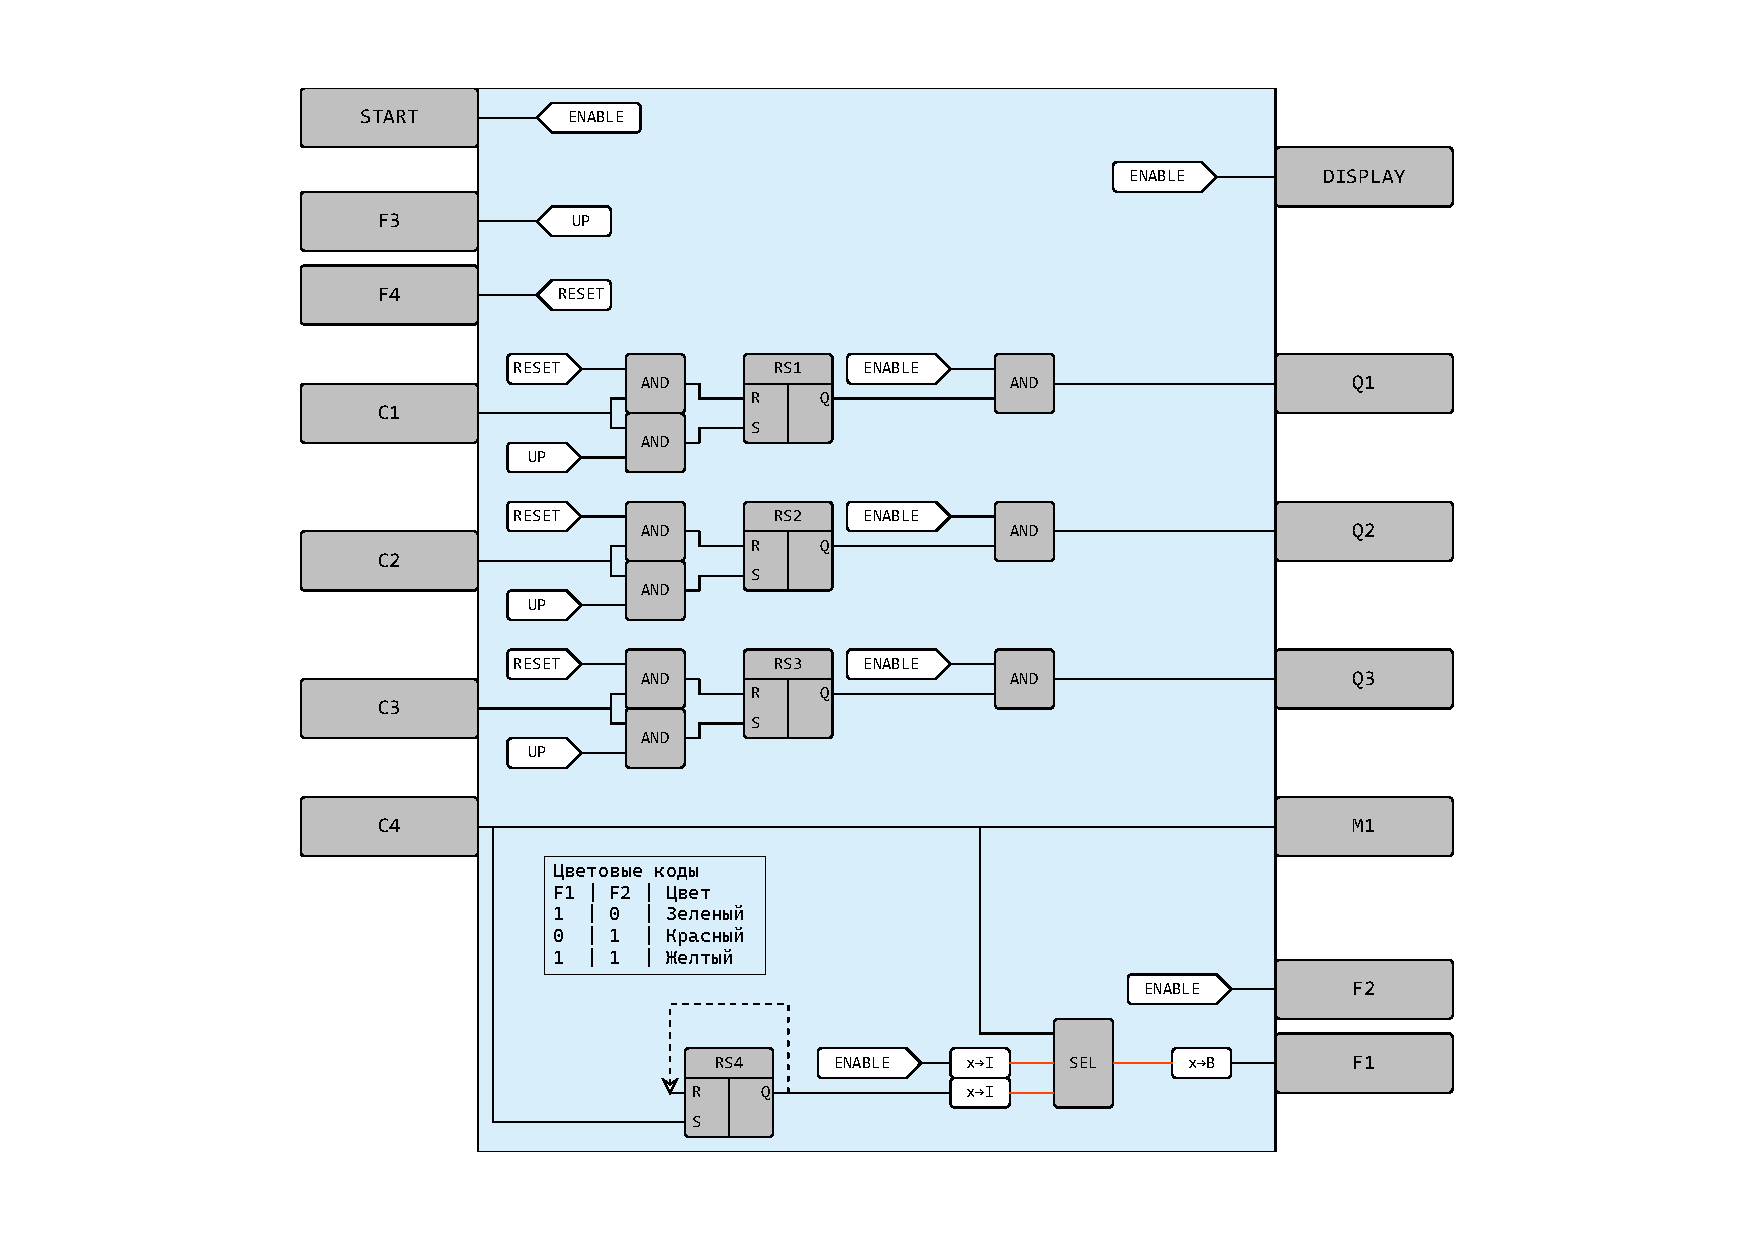
\includegraphics[width=1\textwidth]{fig/manual.pdf}
    \caption{Программа ручного режима}
    \label{fig:manual_mode}
\end{figure}

\begin{figure}[pb]
    \centering
    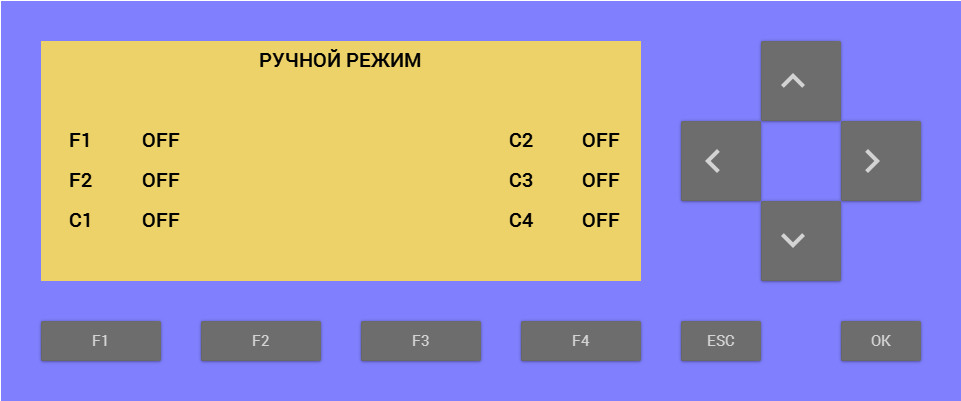
\includegraphics[width=1\textwidth]{fig/manual_panel.png}
    \caption{Экран ручного режима}
    \label{fig:manual_screen}
\end{figure}





%%\clearpage
\section{Робот Rover Vehicle}
\subsection{Обзор робота}
Автомобиль TETRIX PRIME Rover -- это универсальная и увлекательная отправная
точка для различных проектов в области мехатроники и робототехники.
Это наземное транспортное средство, управляемое myRIO и оснащенное
двигателями и датчиками. Вы можете начать, следуя инструкциям по
сборке ровера и запустив предоставленный код. Это позволит вам
удаленно управлять марсоходом для перемещения и захвата объектов с помощью его
эффектора на конце клешни. Вы можете расширить функциональность ровера
, чтобы он мог использовать алгоритмы управления и выполнять задачи.

\subsection{Описание робота}
Два передних колеса приводятся в движение независимо друг от друга двигателями постоянного тока. Заднее колесо используется для балансировки и может свободно вращаться.
Скорость двигателей постоянного тока регулируется с помощью ШИМ, а их направление контролируется с помощью цифровой линии (эта проводка выполняется для вас через плату двигателя).
Ровер имеет дифференциальное рулевое управление, что означает, что направление движения ровера можно изменять, изменяя относительную скорость вращения двигателей постоянного тока.
Данные инфракрасного (ИК) дальномера считываются по аналоговой линии и преобразуются в сантиметры. Его можно использовать для определять расстояние до других объектов или различать различия в цвете и материале на основе ИК-отражательной способности.
Концевой эффектор клещей управляется серводвигателем. Положение серводвигателя контролируется с помощью ШИМ.
AM будет развернут в myRIO, что позволит ему выводить сигналы двигателя, вводить данные датчиков и передавать данные на главный компьютер и с него через сеть WI-Fi.

\newpage
\subsection{Сборка робота}
\begin{figure}[h]
    \begin{subfigure}[b]{0.45\textwidth}
        \centering
        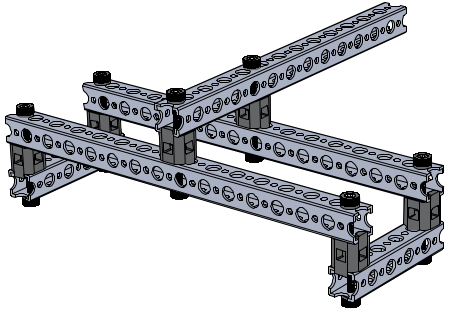
\includegraphics[width=0.7\textwidth]{fig/assembly/1.1.png}
        \caption*{Шаг 1}
    \end{subfigure}
    \begin{subfigure}[b]{0.45\textwidth}
        \centering
        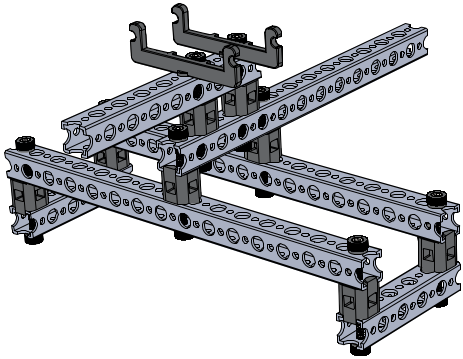
\includegraphics[width=0.7\textwidth]{fig/assembly/1.2.png}
        \caption*{Шаг 2}
    \end{subfigure}
    \begin{subfigure}[b]{0.45\textwidth}
        \centering
        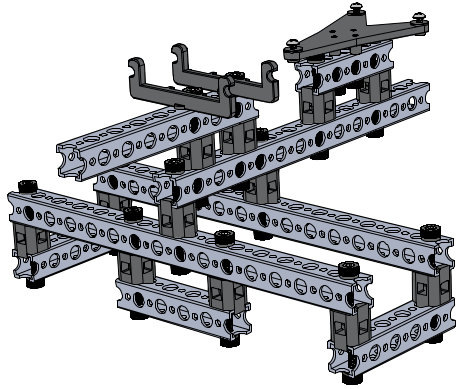
\includegraphics[width=0.7\textwidth]{fig/assembly/1.3.png}
        \caption*{Шаг 3}
    \end{subfigure}
    \begin{subfigure}[b]{0.45\textwidth}
        \centering
        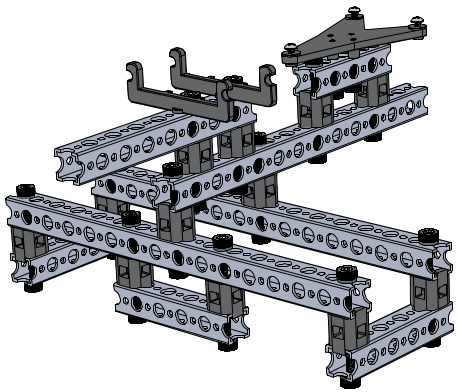
\includegraphics[width=0.7\textwidth]{fig/assembly/1.4.png}
        \caption*{Шаг 4}
    \end{subfigure}
    \begin{subfigure}[b]{0.45\textwidth}
        \centering
        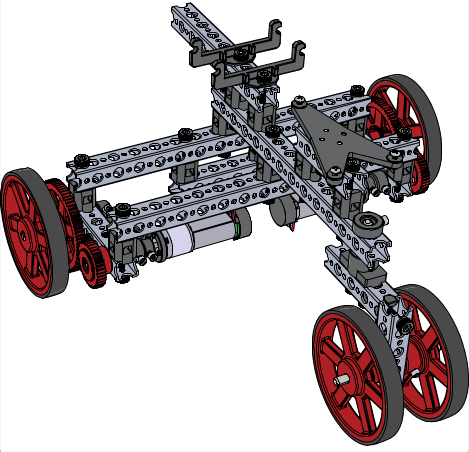
\includegraphics[width=0.7\textwidth]{fig/assembly/1.5.png}
        \caption*{Шаг 5}
    \end{subfigure}
    \begin{subfigure}[b]{0.45\textwidth}
        \flushright
        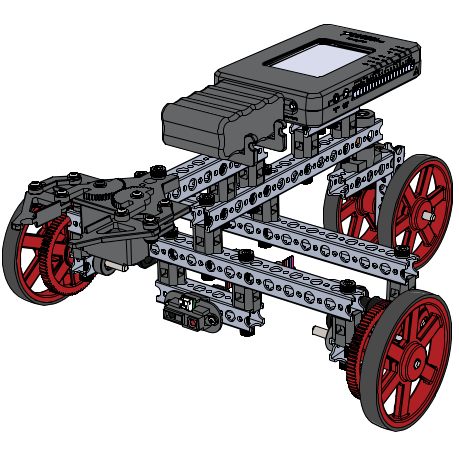
\includegraphics[width=0.7\textwidth]{fig/assembly/1.6.png}
        \caption*{Шаг 6}
    \end{subfigure}
\end{figure}

\newpage
\subsection{Подключение робота}
Подключение робота представлено на рисунке \ref{1connect}.
\begin{figure}[h]
    \centering
    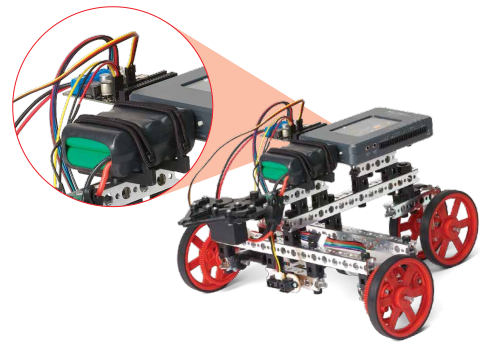
\includegraphics[width=0.7\textwidth]{fig/assembly/1.7.png}
    \caption{Подключение двигателей и периферии}
    \label{1connect}
\end{figure}

\subsection{Испытание робота}
Система управления с замкнутой обратной связью использует контур отрицательной обратной связи с датчиком для измерения выходного сигнала и
сравнения измеренного выходного сигнала, представленного Y (s), с эталонным входом, представленным R (s), для генерации сигнала
ошибки, представленного Ea (s), который управляет контроллер. Если мы сможем надлежащим образом использовать сигнал ошибки, то
достигнем нашей цели отслеживания, то есть сведем к минимуму E(s) =Y(s)-R(s) при наличии внешних помех и установки
неопределенности и изменения параметров. Это ключевая цель разработки контроллера с обратной связью с замкнутым контуром. ИК-датчик
может использоваться для различения цветов на основе различий в отражательной способности ИК-излучения для отслеживания предписанного пути, отмеченного на
земле. Он также может измерять расстояние до препятствий, позволяя нам пропускать препятствия или отслеживать предписанный путь через
загражденную область. С введением датчика мы получаем дополнительный нежелательный шум датчика, представленный
N (s). Основные преимущества управления с замкнутым контуром включают (i) повышенную надежность работы с замкнутым контуром до
изменения параметров установки, (ii) улучшенное подавление внешних помех, ослабление шума измерений
и уменьшение установившейся ошибки системы, и (iii) готовый контроль и регулировка переходной характеристики
системы благодаря умелой конструкции контроллера. Однако эти преимущества сопряжены с затратами. Основная стоимость
управления с обратной связью по замкнутому контуру заключается в дополнительной сложности, что означает более высокие денежные затраты и большую вероятность
отказов компонентов. Поскольку преимущества намного перевешивают недостатки, мы обнаруживаем, что управление с обратной связью по замкнутому контуру широко используется
в современных системах управления. Ключом к управлению с обратной связью по замкнутому контуру является использование сигнала ошибки отслеживания для улучшения
переходной характеристики (время установления, процент превышения и т.д.), а также уменьшения ошибок отслеживания ошибок в установившемся режиме.
Управляющая программа робота представлена на рисунке \ref{1prog}.
\begin{figure}[h]
    \centering
    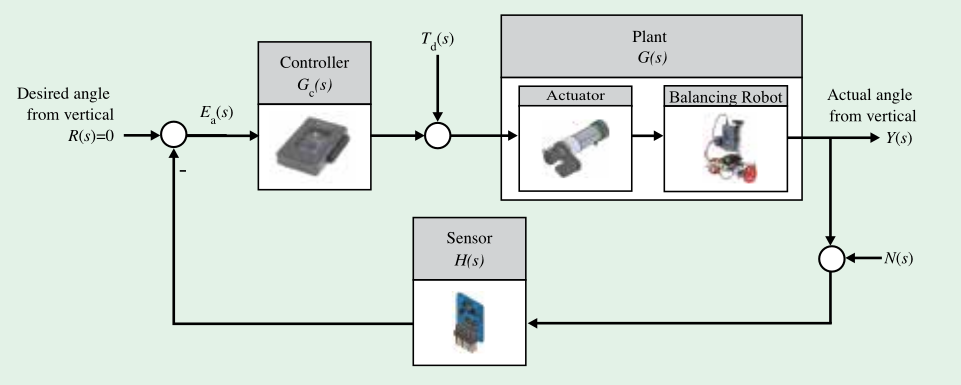
\includegraphics[width=0.7\textwidth]{fig/assembly/1.8.png}
    \caption{Управляющая программа робота}
    \label{1prog}
\end{figure}


%\begin{itemize}
%    \item Если у вас возникли проблемы с отправкой сообщений с вашего хост-компьютера в my ROOM, убедитесь, что IP-адрес на передней панели хост-устройства совпадает с IP-адресом myRIO wireless
%    \item Если ровер движется в неправильном направлении, поменяйте полярность подключения двигателей или активируйте их реверс в программе управления.
%\end{itemize}



%\clearpage
\section{Робот Balancing Arm}
\subsection{Обзор робота}
Балансировочный рычаг TETRIX Prime -- это сборка
, которая демонстрирует, как можно применять концепции управления, преподаваемые
на инженерных курсах. Сама рукоятка
вращается серводвигателем и балансирует
мяч в положении, указанном пользователем (т.е.
заданное значение). Сервопривод управляется
ПИД-регулятором с замкнутым контуром.
Алгоритм, реализован в LabVIEW. Данные
обратной связи - это положение мяча, которое собирается
с инфракрасного (ИК) датчика. Если мяч находится вне
положения, разница между заданным значением
и данными о положении с ИК-датчика (т.е. ошибка)
будет рассчитан, и цикл PID будет корректировать его с течением времени.

\subsection{Описание робота}
Балансировочный рычаг вращается серводвигателем, который получает данные о положении PWM.
Положение мяча измеряется инфракрасным датчиком (ИК), который вводит данные по аналоговой линии.
Пользователь задает заданное значение положения на передней панели LabVIEW VI.
Система постепенно перемещает мяч в нужное положение с помощью ПИД-регулятора.
После сборки пользователь должен откалибровать рычаг, указав положение сервопривода, при котором рычаг
параллелен земле.
Перед каждым использованием пользователь также должен откалибровать контроллер, чтобы распознать минимальные и максимальные края
рычага.
Коэффициенты усиления PID настраиваются автоматически, не требуя ввода пользователем.

\newpage
\subsection{Сборка робота}
\begin{figure}[h]
    \begin{subfigure}[b]{0.45\textwidth}
        \centering
        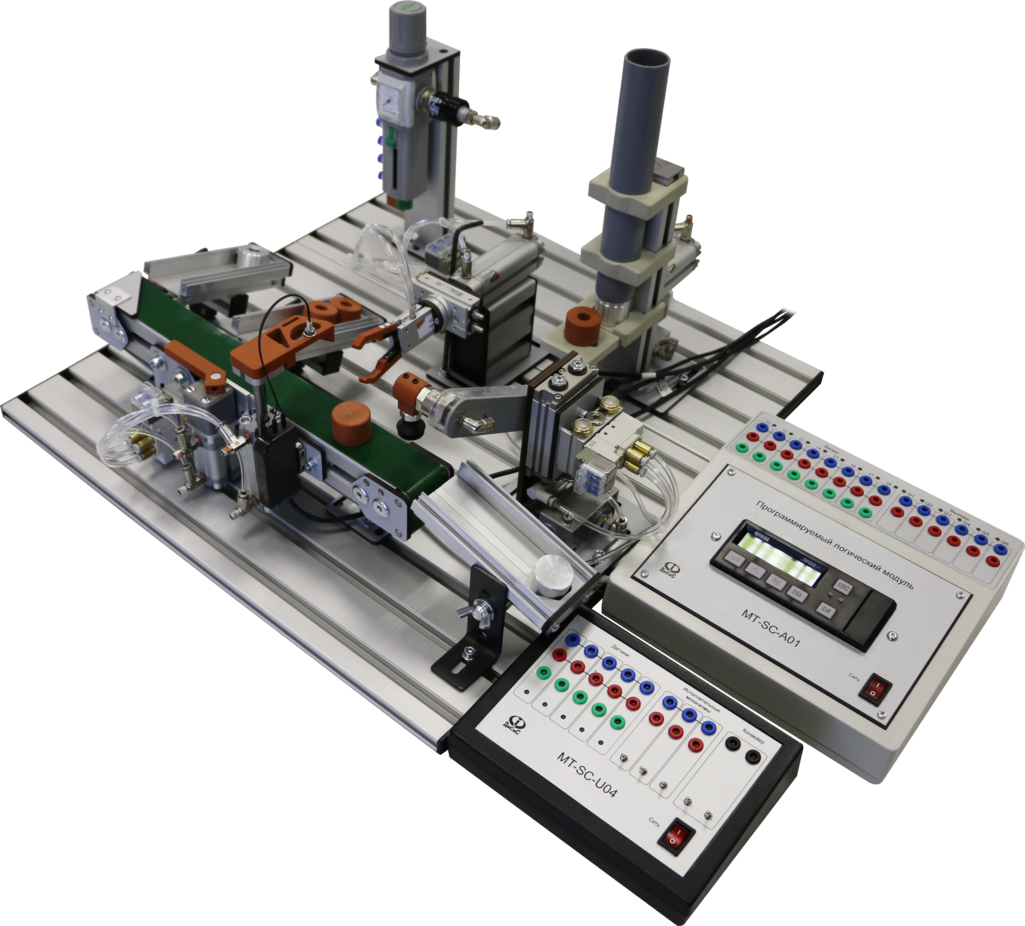
\includegraphics[width=0.7\textwidth]{fig/assembly/2.1.png}
        \caption*{Шаг 1}
    \end{subfigure}
    \begin{subfigure}[b]{0.45\textwidth}
        \centering
        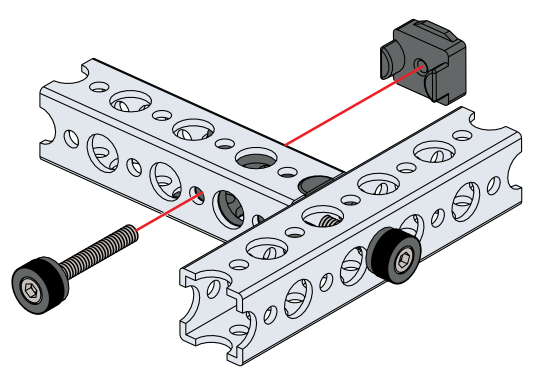
\includegraphics[width=0.7\textwidth]{fig/assembly/2.2.png}
        \caption*{Шаг 2}
    \end{subfigure}
    \begin{subfigure}[b]{0.45\textwidth}
        \centering
        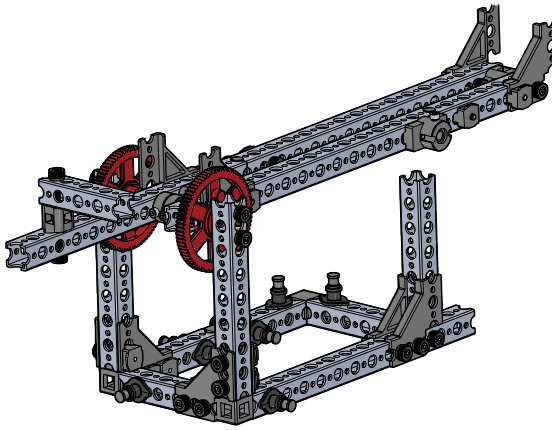
\includegraphics[width=0.7\textwidth]{fig/assembly/2.3.png}
        \caption*{Шаг 3}
    \end{subfigure}
    \begin{subfigure}[b]{0.45\textwidth}
        \centering
        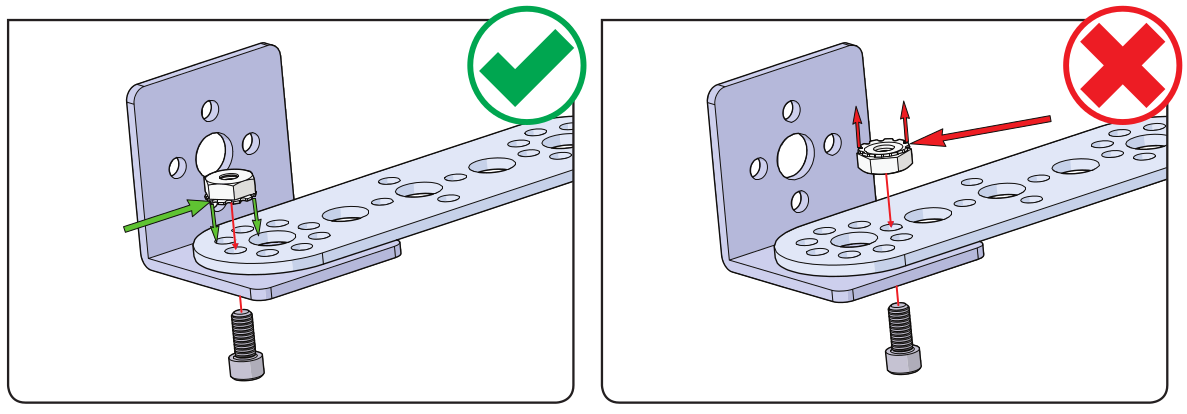
\includegraphics[width=0.7\textwidth]{fig/assembly/2.4.png}
        \caption*{Шаг 4}
    \end{subfigure}
    \begin{subfigure}[b]{0.45\textwidth}
        \centering
        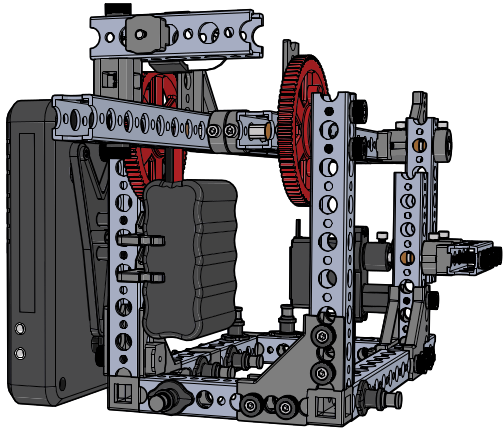
\includegraphics[width=0.7\textwidth]{fig/assembly/2.5.png}
        \caption*{Шаг 5}
    \end{subfigure}
    \begin{subfigure}[b]{0.45\textwidth}
        \flushright
        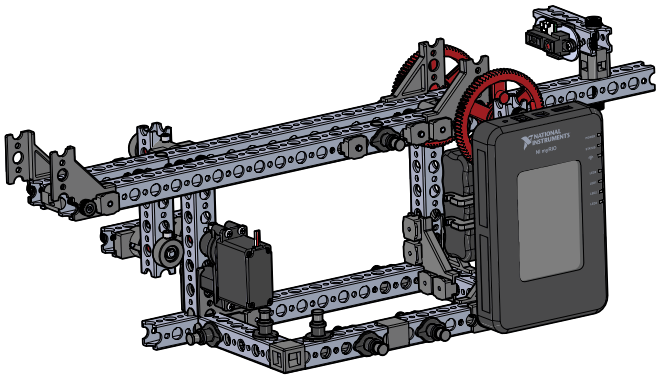
\includegraphics[width=0.7\textwidth]{fig/assembly/2.6.png}
        \caption*{Шаг 6}
    \end{subfigure}
\end{figure}

\newpage
\subsection{Подключение робота}
Подключение робота представлено на рисунке \ref{2connect}.
\begin{figure}[h]
    \centering
    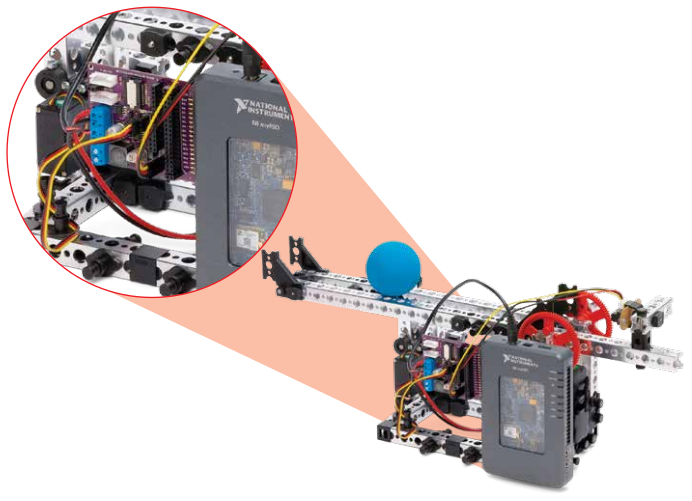
\includegraphics[width=0.7\textwidth]{fig/assembly/2.7.png}
    \caption{Подключение двигателей и периферии}
    \label{2connect}
\end{figure}

\subsection{Испытание робота}
Балансировочный рычаг и один стандартный серводвигатель являются установкой и приводом соответственно. Датчик является
датчиком ИК диапазона и обеспечивает сигнал обратной связи о местоположении мяча относительно датчика, по которому мы можем вычислить
смещение от заданного значения. Команды поступают в систему управления через главный компьютер через
команды передней панели, отправляемые по USB соединению Ethernet на myRIO, на котором размещен код ПИД-регулятора.
Управляющая программа робота представлена на рисунке \ref{2prog}.
\begin{figure}[h]
    \centering
    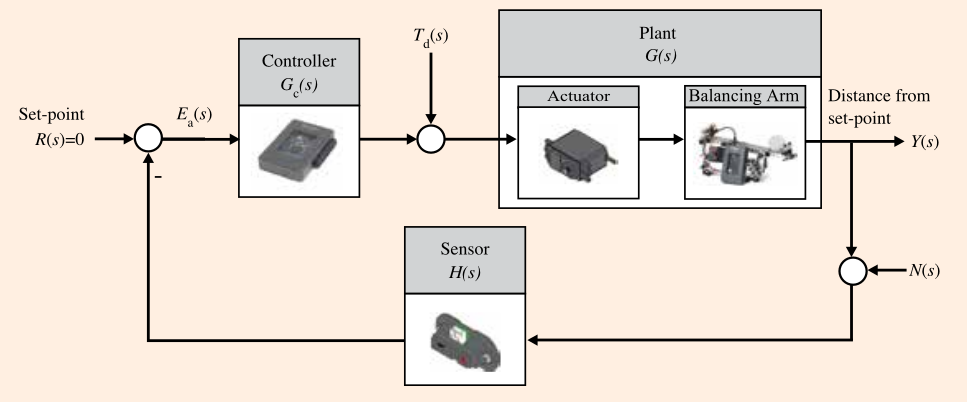
\includegraphics[width=0.7\textwidth]{fig/assembly/2.8.png}
    \caption{Управляющая программа робота}
    \label{2prog}
\end{figure}

%\subsection{Устранение неисправностей}
%\begin{itemize}
%    \item Убедитесь, что стол, за которым вы работаете, ровный и неподвижный
%    \item Убедитесь, что и myRIO, и аккумулятор надежно закреплены в системе, так как их вес способствует устойчивости
%    \item Убедитесь, что ИК-датчик расположен по центру направляющей
%    \item Если электрождвигатели вращаются в неправильном направлении, поменяйте полярность подключения двигателей или активируйте их реверс в программе управления.
%\end{itemize}
%%\clearpage
\section{Робот Self Balancing Robot}
\subsection{Обзор робота}
Самобалансирующийся робот представляет собой сложную систему управления с замкнутым контуром
, которая автономно балансирует себя на месте. Он собирает обратную
связь с нескольких датчиков, включая встроенный акселерометр
myRIO, гироскоп и датчики, встроенные в оба двигателя. Он использует
дополнительный фильтр и PD (пропорционально-дифференциальный) контроллер
в LabVIEW, чтобы стоять вертикально.

\subsection{Описание робота}
Колеса вращаются двигателями постоянного тока, которые работают
независимо и получают данные ШИМ для управления их скоростью.
Датчики, встроенные в каждый двигатель, измеряют относительное
положение и связываются с myRIO с помощью специализированных
цифровых линий кодирования.
Встроенный трехосевой акселерометр myRIO измеряет
статическое и динамическое ускорение.
Гироскоп измеряет скорость вращения и
взаимодействует с myRIO по
протоколу связи I2C.
Дополнительный фильтр используется для обработки данных акселерометра и гироскопа для устранения высокочастотного шума
акселерометр и низкочастотный шум гироскопа.
Регулятор PD используется для управления положением двигателя относительно друг друга.
MyRIO подключается к \\
хост-компьютеру через Wi-Fi.

\newpage
\subsection{Сборка робота}
\begin{figure}[h!]
    \begin{subfigure}[b]{0.45\textwidth}
        \centering
        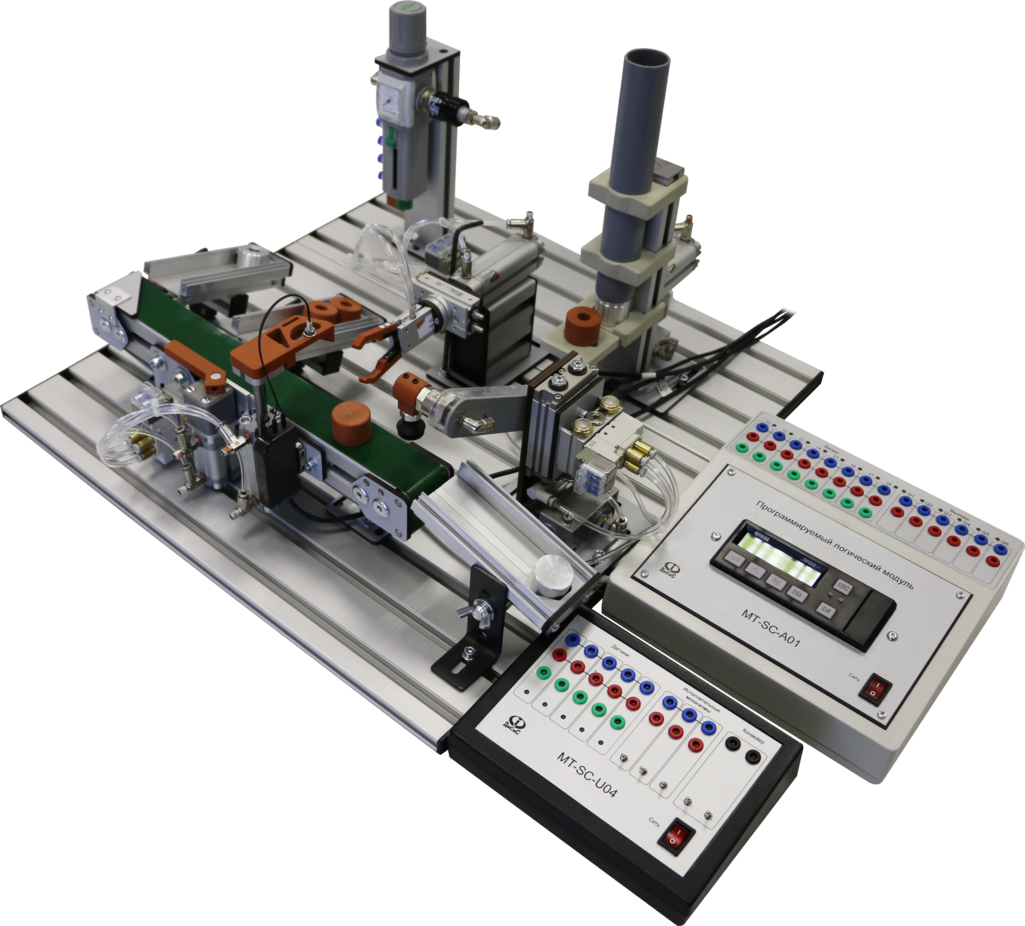
\includegraphics[width=0.7\textwidth]{fig/assembly/3.1.png}
        \caption*{Шаг 1}
    \end{subfigure}
    \begin{subfigure}[b]{0.45\textwidth}
        \centering
        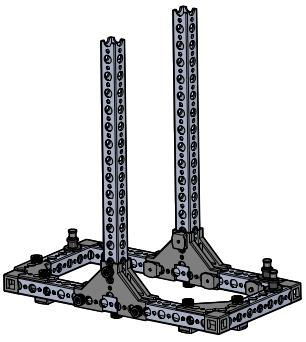
\includegraphics[width=0.7\textwidth]{fig/assembly/3.2.png}
        \caption*{Шаг 2}
    \end{subfigure}
    \begin{subfigure}[b]{0.45\textwidth}
        \centering
        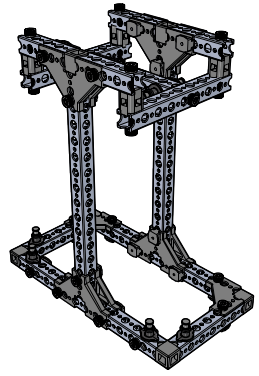
\includegraphics[width=0.7\textwidth]{fig/assembly/3.3.png}
        \caption*{Шаг 3}
    \end{subfigure}
    \begin{subfigure}[b]{0.45\textwidth}
        \centering
        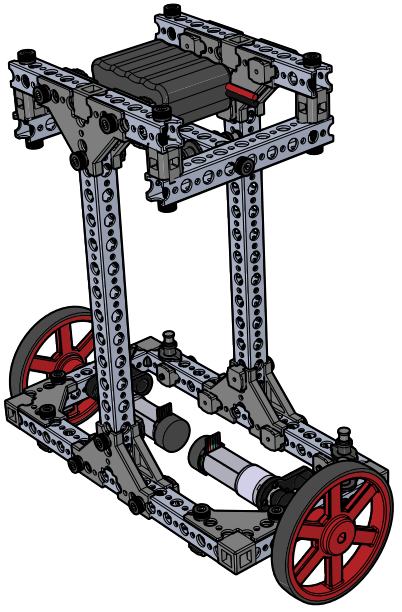
\includegraphics[width=0.7\textwidth]{fig/assembly/3.4.png}
        \caption*{Шаг 4}
    \end{subfigure}
    \begin{subfigure}[b]{0.45\textwidth}
        \centering
        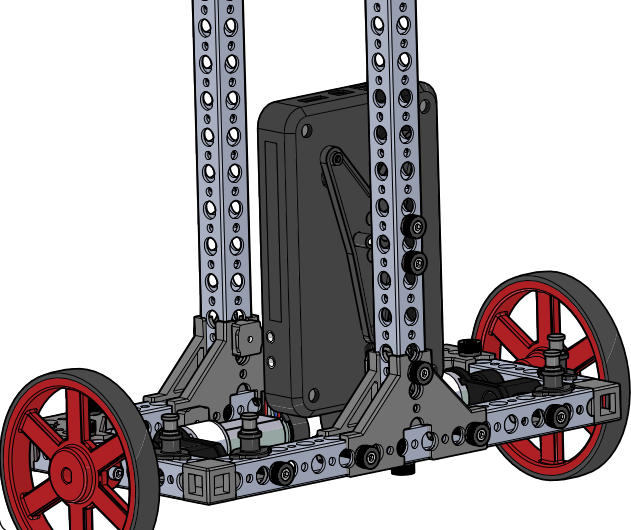
\includegraphics[width=0.7\textwidth]{fig/assembly/3.5.png}
        \caption*{Шаг 5}
    \end{subfigure}
    \begin{subfigure}[b]{0.45\textwidth}
        \flushright
        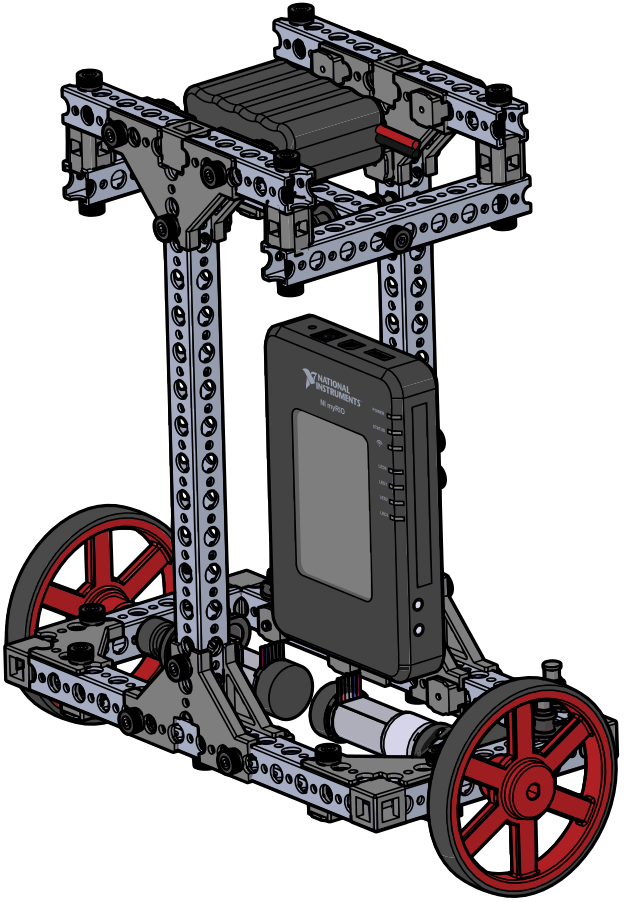
\includegraphics[width=0.7\textwidth]{fig/assembly/3.6.png}
        \caption*{Шаг 6}
    \end{subfigure}
\end{figure}
\clearpage

\newpage
\subsection{Подключение робота}
Подключение робота представлено на рисунке \ref{3connect}.
\begin{figure}[h]
    \centering
    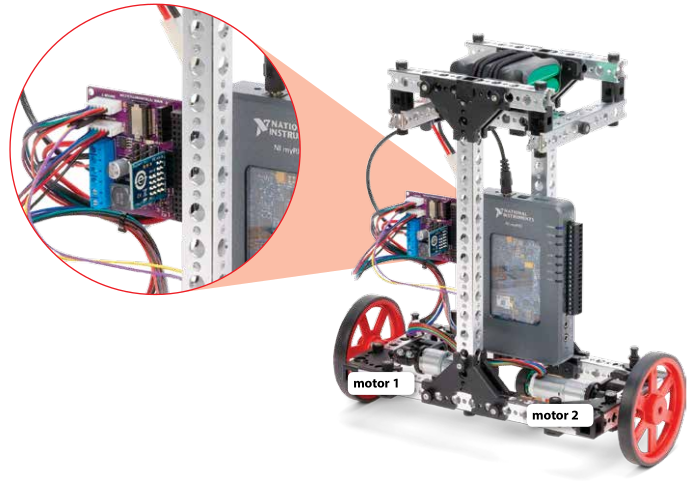
\includegraphics[width=0.5\textwidth]{fig/assembly/3.7.png}
    \caption{Подключение двигателей и периферии}
    \label{3connect}
\end{figure}

\subsection{Испытание робота}
Самобалансирующийся робот и два зубчатых колеса с приводом от двигателя постоянного тока являются установкой и исполнительными механизмами соответственно. Набор датчиков
включает в себя гироскоп, который измеряет угловую скорость, и акселерометр, который измеряет негравитационное
ускорение. Поскольку известно, что акселерометр и гироскоп имеют систематические ошибки и зашумлены,
сигналы от датчиков объединяются для получения точного измерения угла ориентации робота —
более точного, чем может быть достигнуто с помощью любого датчика по отдельности. Команды внешней ссылки вводят
Цель конструкции - уравновесить робота в вертикальном
положении при наличии внешних помех и обеспечить его надежную устойчивость к колебаниям растений. Контроллер - это контроллер PD.
Управляющая программа робота представлена на рисунке \ref{3prog}.
\begin{figure}[h]
    \centering
    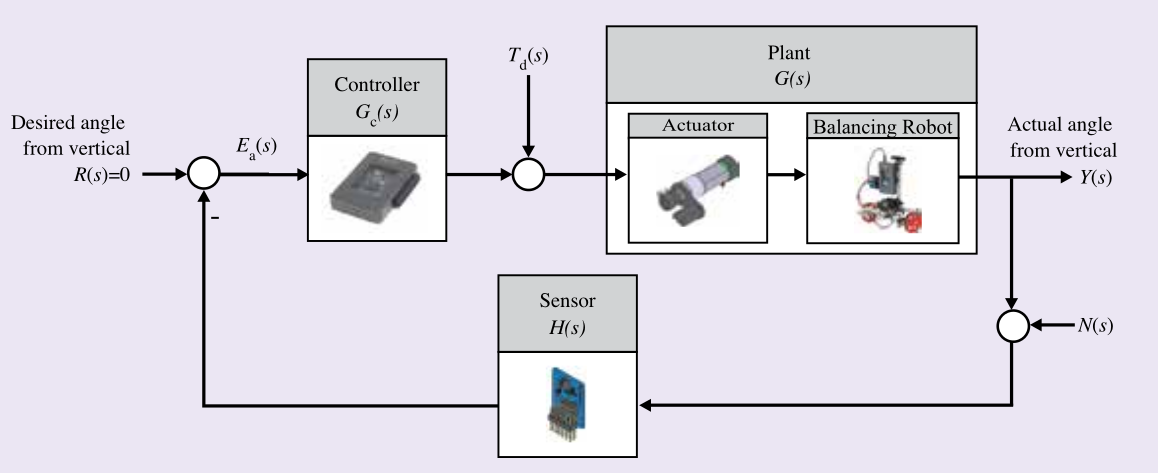
\includegraphics[width=0.4\textwidth]{fig/assembly/3.8.png}
    \caption{Управляющая программа робота}
    \label{3prog}
\end{figure}

%\subsection{Устранение неисправностей}
%\begin{itemize}
%    \item Дважды проверьте, правильно ли подключены двигатели и энкодер -- если их поменять местами, робот не будет балансировать
%    \item Если вы возьмете в руки самобалансирующегося робота или нажмете на него слишком сильно, то может сбиться калибровка. Для возвращения робота в рабочее состояние проведите повторную калибровку. Нажмите кнопку 0 в нижней
%    части myRIO, чтобы выключить колеса и систему управления, а затем проведите калибровку, чтобы снова сбалансировать его. Процедура калибровки выглядит следующим образом:
%    \begin{itemize}
%        \item Держите робота вертикально так, чтобы его центральная линия была перпендикулярна земле
%        \item Нажмите <<Button 0>> в нижней части myRIO, все еще удерживая робота вертикально, и быстро отпустите
%    \end{itemize}
%\end{itemize}
